\documentclass{article}
\usepackage{tikz}
\newcommand{\boxprobe}[3]{\setbox0=\hbox{#2#3}\typeout{BOX #1: \the\wd0,\the\ht0,\the\dp0}}
\newcommand{\anchorprobe}[2]{\pgfextractx{\dimen0}{\pgfpointanchor{#1}{#2}}\pgfextracty{\dimen2}{\pgfpointanchor{#1}{#2}}\typeout{POINT #1.#2: \the\dimen0,\the\dimen2}}
\begin{document}
\boxprobe{prose}{}{Koordinatenfrei}
\boxprobe{descenders}{}{gyjp}
\boxprobe{measurements}{}{measurements}
\boxprobe{small}{\scriptsize}{measurements}
\boxprobe{bold}{\large\bfseries}{Mixed ABC}
\boxprobe{tiny}{\tiny}{tiny capitals}
\boxprobe{equals}{}{=}
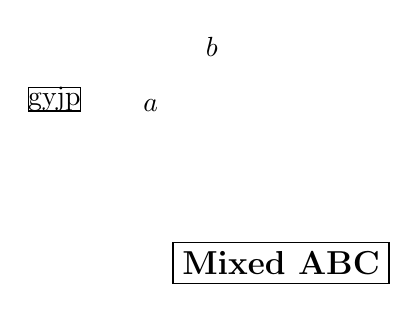
\begin{tikzpicture}
  \node[draw,inner sep=0pt,anchor=base] (a) at (0,1) {gyjp};
  \node[draw,font=\large\bfseries,anchor=west] (b) at (1.5,-1) {Mixed ABC};
  \node[anchor=west,xshift=0.2] (c) at (1,1) {$a$};
  \node[anchor=north,yshift=-0.1] (d) at (2,2) {$b$};
  \anchorprobe{a}{base}\anchorprobe{a}{center}
  \anchorprobe{b}{center}\anchorprobe{b}{base west}
  \anchorprobe{c}{center}\anchorprobe{d}{center}
\end{tikzpicture}
\end{document}
